\section{Additional background}
Learning curves - see pattern book


\section{General for the three models}
%Additional info that need to be placed somewhere. 
%\begin{itemize}
%\item There are simple methods that can be used to improve performance and training speed. Scaling of the input and giving an initial weight \citep{Duda2000}
%\end{itemize}

For all the models the input and hidden layers uses the ReLu activation, since this is the most common used in neural network. \citep{Goodfellow2016} %Maybe the grid test suport ths as well, and maybe also something about computation power. 

and the sigmoid for the output layer.  




%TEMP CRAP THAT NEEDS TO BE PLACED ELSEWHERE
Temp-placehoder:
The process of making the neural network model has been a trial and error process, because there is not an actual “cookbook” for developing NN (This statement is from a not vaild source, but so far it’s the only one that i have found.)  

\subsection{Data-handling in python}
The preprocessed data save as a .mat file which is loaded into python. Before splitting the data into different sub-sets, it is shuffled to ensure generalization through randomization. The data is then split into a training-set and a test-set, and respectively makes out 85 \% and 15 \% of the preprocessed data. \textbf{NEED A SOURCE OR A ARGUMENT FOR WE SPLIT THE DATA LIKE THIS.} The test-set will only be used to evaluate the generalization of the model, and therefore won't contain data that's been used during training \citep{Duda2000}. 
By keeping the test-set separate will act as new unseen data, for the model.  

The training-set is additionally split into a another training-set and a validation-set. Here the new training-set makes out 90 \% of the sub-set and the validation set is the remaining 10 \%. \textbf{WE NEED A SOURCE/OR A GOOD ARGUMENT FOR THIS, SAME AS ABOVE} 
The validation set will be used to estimate the generalization error during training \citep{Duda2000}.  

\subsection{Applied optimization techniques}
To reduce overfitting and to optimize the network different techniques are applied to the different network models. The result of this is hoped to be better generalization of the models. 

\subsubsection{Dropout}
Dropout is a technique that can be used to prevent or reduce overfitting of a neural network. In a network the dropout can be applied to the individual layers, and works by randomly drop/”turn off” different nodes temporarily in the given layer during training. An illustration of the principle of dropout can be seen in \autoref{fig:Dropout}.  

\begin{figure} [H]
\centering
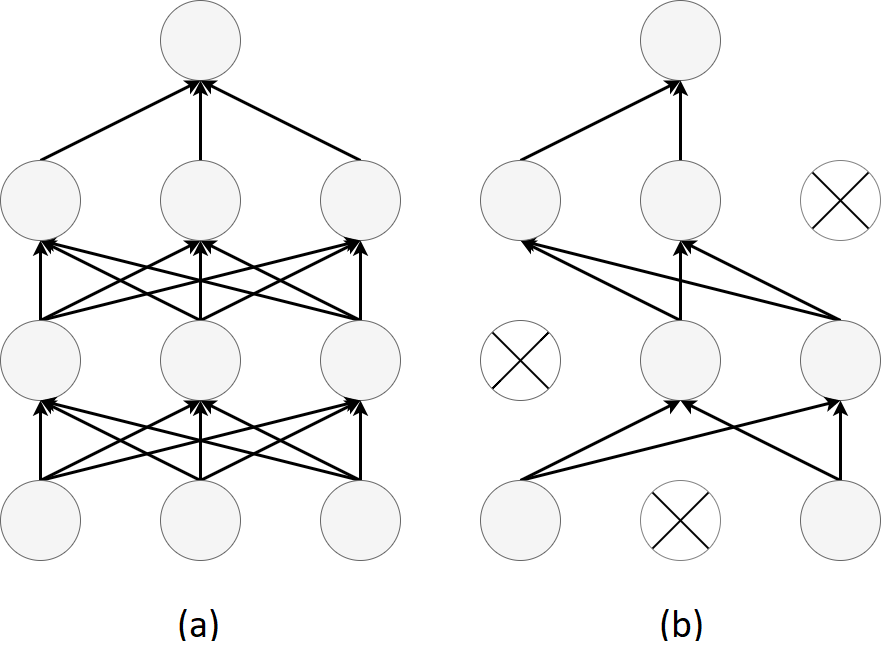
\includegraphics[width=0.6\textwidth]{figures/Dropout}
\caption{Illustration of dropout effect: The figure on the left illustrates a fully connected network, without dropout, and the right shows a network where dropout is enabled on the first three layers.}
\label{fig:Dropout}  
\end{figure}

This reduces co-adaptation, where nodes compute the same features, to where this may increase the generalisation capabilities for a neural network.\citep{Srivastava2014}  
A study, has tested the use of dropout in different neural networks, and indicates that the most optimal range of dropout is 20 \% of the nodes in the visible layers, and 50 \% in the hidden layers \citep{Srivastava2014}.
When implementing dropout to the models, it is defined in the given layers, and specified with a float value between 0 and 1, which defines the fraction of the nodes that drop \citep{Chollet2015}.



\subsubsection{Kernel-initializer 'Maybe'}
This is a must i think because this relates to the reproducible aspect. 

\subsubsection{Learning rate 'Maybe'}
A must because we have done this. 

\subsubsection{Training with noise 'Maybe'}
NO GONNA HAPPEN, but it was a method mentioned the pattern recognition book

\subsubsection{Manufacturing data 'Maybe'}
I don't think this is gonna be a reality 

\subsubsection{Batch training}
Save computational cost, update parameters when a batch has been trained. 
 
\subsubsection{Grid testing 'Maybe'}
MAYBE SOMETHING ABOUT GRID TESTING if we can make it reproductive
OBS can only use images as an input

 
 
\subsection{Training of the networks}
Supervised learning is used for training in all the models. The generic input for all of the model is gender, along with the different image representation, which are described in \autoref{BIRGITHE&LINETTE}. These inputs trained and then compared against their respective category label.   
The models classify data into three different classes e.g. duration interval of 0-12 months, 18-30 months and 36 months and above. Because of this multi classification, the output labels are changed from integer representation, 0 (0-12 months), 1 (16-30 months) and 2 ( and 36 months and above) into a one-hot encoded representation [0 , 0 , 1], [0 , 1 , 0] and [1 , 0 , 0] respectively. This is done by using keras utility function called \textit{to_categorical}. 

\subsubsection{Cross-validation}
Because the amount of data for this project is limited it is chosen to implement m-fold cross validation, where the training data is divided into m number of subsets. Each of the subsets can function a either a validation set or as a part of a training set e.g. if a classifier is trained \textit{m} times, then each time a different subset will be used as a validation set, and the rest is used for training. \citep{Duda2000}
Because of the property of cross validation, it can be used as a way of improving generalization accuracy since all data is included during training, but may not be beneficial for every kind of problem. \citep{Duda2000}

\section{Vector image model}
The architecture for this model only contains fully connected layer, since the data representation only contains 21 element vector that reflects the active pain regions and gender as described in \autoref{LinetteAndBirgithe}. It's evaluated that there wouldn't be any gains in making the model more complex e.g. adding of convolution, based on the information available from vector, since the level of detail in relation to morphology is very simple. 
The architecture of the model is illustrated in \autoref{fig:simpleModel}. 

\begin{figure} [H]
\centering
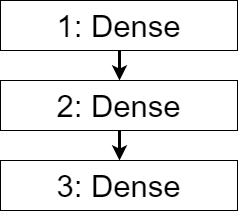
\includegraphics[width=0.6\textwidth]{figures/simpleModel}
\caption{Arcitechture of the neural network using knee region representation.}
\label{fig:simpleModel}  
\end{figure}

The model consists of three layers, where the input and output layer... 




\section{Raw binary representation model}\label{sec:binaryRepModel}
The architecture of this model is based on the typical structure of a convolutional network, where the first layers alternate between convolutional layers and max pooling layers \citep{LeCun2015}. This defines the first part of the model. The following layers consists of three fully connected layers, and output layer, and defined the second part of the model. An overview of the architecture is shown in \autoref{fig:binaryRepModel}.  
Convolution layer are implemented for this pain map representation, because of their ability to extract morphology features from images, as written in \autoref{CONVOLUTION}

\begin{figure} [H]
\centering
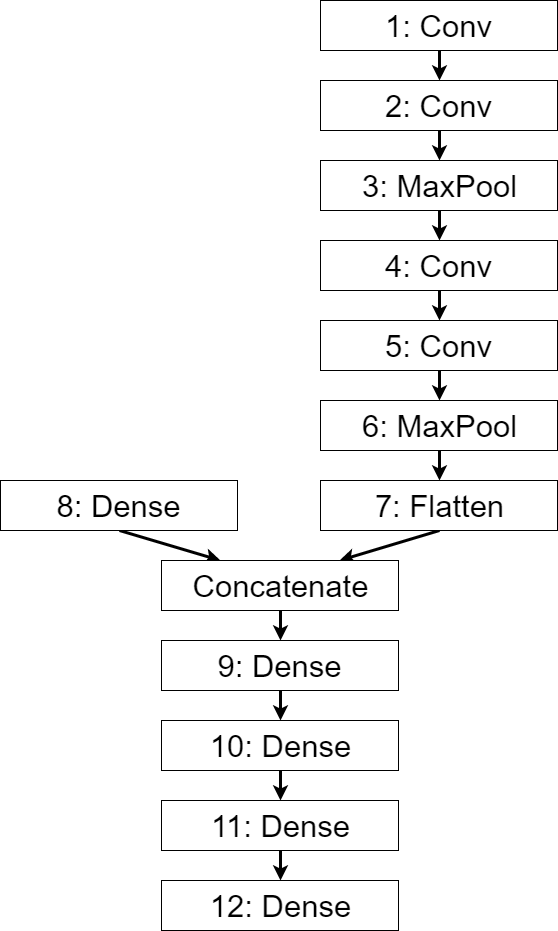
\includegraphics[width=0.6\textwidth]{figures/binaryRepModel}
\caption{Architecture for the neural network model using binary pain map representation. REMEMBER TO INCLUDE THE INPUT IN THE FIGURE}
\label{fig:binaryRepModel}  
\end{figure}

Rather then feeding both pain map representation and gender into the same input layer, they are separated and used as input at two different locations. 
The binary pain map representation works as input in first part of the model, where the input layer is a convolution layer. 
This layer is setup to receive a input shape to that of the dimension of the pain map, that is defined during re-scaleing of the pain maps in \ref{LINETTE&BIRGITHE}. 
Gender works as secondary input in the second section of the model, along with the pain maps features extracted through the convolution layers. Before the pain maps features reach the fully connected part of the network it is flattened from a matrix to a single row in order to merge the features with gender. 
The merged data passes the fully connected layers and reaches the output layer where it is given a percentage value according to which class it fits the most. 


THIS NEEDS TO BE REWRITTEN: The reason for separating gender and binary images is given as separate inputs is because of that there is no benefit in feeding gender through several convolutional layers, since these layer are use for looking at the shapes of the pain.  

The reason for using gender as input this far into the model, is a result of the way that convolution works 



\section{Combined model}
The architecture of this model is nearly identical to that of the binary representation model as described in \ref{sec:binaryRepModel}. 
The main difference can only be seen in the input layer for the pain map representation, where the input shape is altered to contain 20 layers per pain maps instead of one. 
This is the result of the one hot encoding done to the images as described in \autoref{LinetteAndBirgithe}. 

